% !TeX root = ../paper.tex
\section{Data Construction and Annotation Details}
\label{appendix:data-construction}

This appendix details the data construction method in
Section~\ref{steering-oriented-data-construction},
including data sources, quality filtering and unified representations,
action-first segmentation, grade-conditioned annotation, instruction
rewriting, and exported data statistics.

\hypertarget{raw-trajectory-sources}{%
\subsection{Raw Trajectory Sources}\label{raw-trajectory-sources}}

The raw trajectory pool consists of DROID~\citep{khazatsky2024droid},
MolmoAct~\citep{lee2025molmoact}, AgiBot-World~\citep{agibot2025world}, and
RH20T~\citep{fang2023rh20t}. DROID contains large-scale single-arm Franka teleoperation data
collected across real scenes, with 76K trajectories, 564
scenes, and 86 tasks. MolmoAct contains 10,689 high-quality single-arm
Franka trajectories over 93 household and tabletop tasks. AgiBot-World
provides million-scale real-robot data, including
1,001,552 trajectories, 217 tasks, and 87 skill
categories. RH20T contains more than 110K contact-rich robot
manipulation sequences with human-operation videos or demonstrations;
its task collection comprises 147 tasks. Table~\ref{tab:raw-sources} reports the complete public
scale of each
dataset, not the number retained or segmented by SmartVLA; those counts
are reported separately below.

% !TeX root = ../paper.tex
\begingroup
\normalsize
\setlength{\tabcolsep}{4pt}
\setlength{\LTcapwidth}{\linewidth}
\setlength{\LTpre}{\baselineskip}
\setlength{\LTpost}{\baselineskip}
\renewcommand{\arraystretch}{1.10}
\begin{longtable}[]{@{}
  >{\raggedright\arraybackslash}p{(\columnwidth - 6\tabcolsep) * \real{0.18}}
  >{\raggedleft\arraybackslash}p{(\columnwidth - 6\tabcolsep) * \real{0.25}}
  >{\raggedleft\arraybackslash}p{(\columnwidth - 6\tabcolsep) * \real{0.15}}
  >{\raggedright\arraybackslash}p{(\columnwidth - 6\tabcolsep) * \real{0.42}}@{}}
\caption{Public raw trajectory sources used to construct the training pool.}\label{tab:raw-sources}\\
\toprule\noalign{}
\begin{minipage}[b]{\linewidth}\raggedright
Dataset
\end{minipage} & \begin{minipage}[b]{\linewidth}\raggedleft
Public raw trajectories / sequences
\end{minipage} & \begin{minipage}[b]{\linewidth}\raggedleft
Tasks
\end{minipage} & \begin{minipage}[b]{\linewidth}\raggedright
Collection coverage
\end{minipage} \\
\midrule\noalign{}
\endhead
\bottomrule\noalign{}
\endlastfoot
DROID & 76K & 86 tasks & 564 scenes; single-arm Franka \\
MolmoAct & 10k & 93 tasks & home and tabletop; single-arm
Franka \\
AgiBot-World & 1,001k & 217 tasks & 106
scenes; 100 real robots \\
RH20T & 110K & 147 tasks & 7 configurations
across 4 robot types \\
\end{longtable}
\endgroup
%

\hypertarget{pipeline-overview}{%
\subsection{Pipeline Overview}\label{pipeline-overview}}

The SmartVLA pipeline decomposes the conversion from raw trajectories to
trainable steering supervision into seven stages. We first filter and
canonicalize data across sources, then use action and visual evidence to
determine boundaries, object locations, and spatial cues, and finally
generate replaceable instruction rewrites. The complete stage mapping is
shown in Table~\ref{tab:pipeline}.

The pipeline separates trajectory analysis, instruction generation, and consistency review. Action
and visual evidence first define segment records containing control phases, object roles, and
spatial candidates. Grade-conditioned rules then restrict instruction generation to descriptions
appropriate for those records, and the review stage removes inconsistent language or spatial labels.
This organization reuses existing demonstrations and grounds language generation in structured
evidence, rather than requiring unconstrained descriptions to determine the full temporal structure.

Figure~\ref{fig:appendix-action-aligned-pipeline} illustrates these operations
using an RH20T demonstration of slicing lotus root with a knife. The
segment-level examples show how one task yields distinct local requirements:
approaching and grasping the knife, transferring and aligning it, slicing,
and withdrawing. Each segment receives applicable language rewrites and
visual prompts tied to its behavior and target, rather than inheriting the
same complete-task description. High-interaction segments retain task and
visual-prompt rewrites without object-free atomic-motion variants.

% !TeX root = ../paper.tex
\begin{figure}[!t]
\centering
\setlength{\parskip}{0pt}
\setlength{\abovecaptionskip}{\baselineskip}
\setlength{\belowcaptionskip}{0pt}
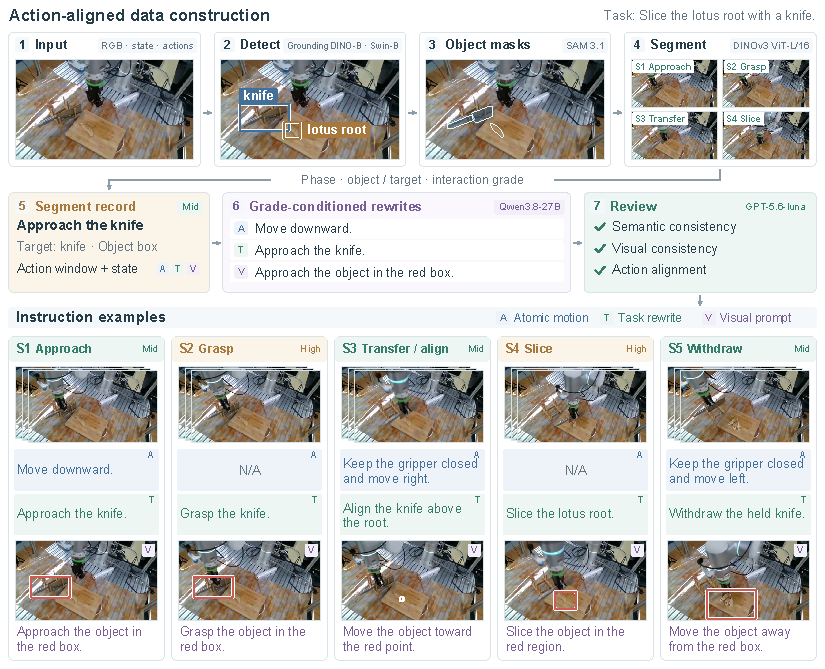
\includegraphics[width=\textwidth]{figures/appendix_action_aligned_pipeline_v12.pdf}\par\nointerlineskip
\caption{Action-aligned data construction illustrated with an RH20T
knife-and-lotus-root demonstration. Top: visual evidence extraction,
action-aligned segmentation, segment recording, grade-conditioned rewriting,
and consistency review. Bottom: atomic-motion (A), task-language (T), and
visual-prompt (V) examples for approach, grasp, transfer/alignment, slicing,
and withdrawal. N/A indicates that atomic-motion rewriting is excluded for
High-interaction segments.}
\label{fig:appendix-action-aligned-pipeline}
\end{figure}
%

% !TeX root = ../paper.tex
\begingroup
\normalsize
\setlength{\tabcolsep}{4pt}
\setlength{\LTcapwidth}{\linewidth}
\setlength{\LTpre}{\baselineskip}
\setlength{\LTpost}{\baselineskip}
\renewcommand{\arraystretch}{1.10}
\begin{longtable}[]{@{}
  >{\raggedright\arraybackslash}p{(\columnwidth - 6\tabcolsep) * \real{0.20}}
  >{\raggedright\arraybackslash}p{(\columnwidth - 6\tabcolsep) * \real{0.28}}
  >{\raggedright\arraybackslash}p{(\columnwidth - 6\tabcolsep) * \real{0.32}}
  >{\raggedright\arraybackslash}p{(\columnwidth - 6\tabcolsep) * \real{0.20}}@{}}
\caption{Seven-stage steering-oriented data construction pipeline.}\label{tab:pipeline}\\
\toprule\noalign{}
\begin{minipage}[b]{\linewidth}\raggedright
Stage
\end{minipage} & \begin{minipage}[b]{\linewidth}\raggedright
Main evidence
\end{minipage} & \begin{minipage}[b]{\linewidth}\raggedright
Operation
\end{minipage} & \begin{minipage}[b]{\linewidth}\raggedright
Output
\end{minipage} \\
\midrule\noalign{}
\endfirsthead
\toprule
Stage & Main evidence & Operation & Output \\
\midrule
\endhead
\bottomrule\noalign{}
\endlastfoot
A. Filtering and normalization & language labels, video decodability,
image quality, state/action statistics & remove unlabeled, low-quality,
or noisy samples and unify image, state, and action formats & valid
trajectories in a canonical format \\
\midrule
B. Candidate boundary generation & action increments, action curvature,
gripper events, visual changes, detection and segmentation & extract
candidate peaks from action/visual curves and merge overly short
segments by temporal smoothing & candidate control segments \\
\midrule
C. Interaction evidence modeling & object masks and tracks,
gripper-to-target distance, contact evidence, object motion, gripper
state & infer active object, target region, contact relation, and
control relevance & interaction curves and spatial candidates \\
\midrule
D. Action-first refinement & intermediate records from B/C, task-family
priors, action segments & refine boundaries, assign a segment grade, and
bind semantic actions to object relations & action-aligned segment
records \\
\midrule
E. Grade-conditioned rewriting & segment grade, original task, action
primitive, object/target roles, visual/spatial evidence & select
applicable rewrite families by grade and generate candidates &
grade-organized rewrite pool \\
\midrule
F. Rewrite sampling metadata & task type, phase, rewrite family, segment
grade & record recommended sampling weights and applicability conditions
& typed rewrite pool with sampling metadata \\
\midrule
G. VLM review and expansion & keyframes, rewrite candidates, spatial
candidates & review spatial cues and language rewrites, add constrained
expressions, and disable unreliable labels & reviewed segment
annotations \\
\end{longtable}
\endgroup
%

This decomposition exposes auditable intermediate products. Incoming
trajectories pass language, image, action-quality, and canonical-schema
checks; boundaries come from action and visual curves; spatial cues come
from detection, segmentation, tracking, motion, and contact evidence;
and rewrites come from constrained segment records. The final output is
not a single caption but two complementary forms of supervision: one
describes phase sub-tasks, atomic motions, object roles, and relational
constraints, while the other encodes visible targets, regions, and
motion trajectories as multimodal inputs. Every training example can be
traced to a source segment, interaction evidence, and rewrite type.

\hypertarget{filtering-and-canonical-normalization}{%
\subsection{Filtering and Canonical
Normalization}\label{filtering-and-canonical-normalization}}

We first perform quality filtering. We remove three categories of
unlearnable or highly noisy samples. First, episodes or spans without
language labels or with empty task text cannot provide a stable
instruction anchor. Second, we remove poor visual data, including
undecodable videos, black or corrupted frames, severe blur, missing key
views, camera jumps, and targets that remain invisible for an extended
period. Third, we remove poor actions, including missing state/action
values, NaNs or out-of-range actions, long idle periods, clear
video-action desynchronization, failed initialization, abnormal gripper
state, and trajectories that are too short.

After filtering, action-first segmentation processes only trajectories
with readable task language, usable visual observations, and learnable
action signals. We map each source to a common multimodal control
format. Every sample contains a third-person view and the wrist view of
the currently active arm: single-arm trajectories retain one wrist view,
while bimanual trajectories retain left and right wrist views
separately; side and auxiliary views are retained when available.

To support both single-arm and bimanual embodiments, we use fixed
32-dimensional state and action containers and record embodiment type,
active arm, and a valid-dimension mask for every sample. Single-arm data
occupies one arm slot. Bimanual data such as AgiBot-World writes the
left and right arm state/action into independent slots. Each arm slot
primarily represents end-effector pose, gripper state, and relative
end-effector action. Base, waist, joint, force, and other information is
stored in reserved dimensions or retained as auxiliary proprioception.
Padding dimensions unused by the current embodiment do not contribute to
the training loss.

Action normalization is also performed at this stage. We prioritize
available end-effector poses, Cartesian actions, or end-effector poses
reliably computed by forward kinematics. Absolute end-effector targets
are converted into increments relative to the current state, while
native end-effector increments retain their control semantics and are
reordered into a common axis convention. Normalization statistics are
computed per data source and embodiment configuration over valid state
and action dimensions, including means, standard deviations, quantiles,
and clipping ranges. Different sources therefore share tensor interfaces
and dimension semantics while retaining the true scale and control
distribution of each robot.

\hypertarget{action-first-segmentation}{%
\subsection{Action-First Segmentation}\label{action-first-segmentation}}

SmartVLA derives segment boundaries from action and visual evidence
rather than free-form descriptions from a language model. We compute
adjacent action-vector differences, action curvature, gripper
opening/closing events, embedding shifts in third-person and wrist
views, and changes in open-vocabulary object observations. Candidate
boundaries are merged into segments using temporal smoothing and
task-family rules. This aligns each action segment with a local control
phase, rather than binding an episode-level caption to every timestep.

We use DINOv3 ViT-L/16 to compute cross-frame visual changes,
GroundingDINO-B with a Swin-B backbone to localize candidate objects in
keyframes, and SAM~3.1 to obtain object or target-region masks.
Point/box trackers and temporal consistency checks propagate locations
through the trajectory. Because the detector requires text queries, we
extract names of manipulated and target objects from the original
instruction and augment them with descriptions implied by the candidate
segment phase. We then combine gripper-to-target distance, contact
evidence, object motion, and gripper state to infer the active object,
target region, and interaction phase for each segment.

The resulting action segments provide local steering supervision,
while original-task examples retain their continuous
demonstration trajectories. Unused embodiment dimensions remain masked as
described above.

\hypertarget{grade-conditioned-steering-instruction-rewriting}{%
\subsection{Grade-Conditioned Steering Instruction
Rewriting}\label{grade-conditioned-steering-instruction-rewriting}}

Each record stores the action segment, its control phase, interaction
grade, and available object and spatial evidence. The grade selects among
the three rewrite families defined in Section~\ref{steering-oriented-data-construction},
rather than filtering segments. Table~\ref{tab:rewrite-policies} associates
typical phases with the permitted families.

% !TeX root = ../paper.tex
\begingroup
\normalsize
\setlength{\tabcolsep}{4pt}
\setlength{\LTcapwidth}{\linewidth}
\setlength{\LTpre}{\baselineskip}
\setlength{\LTpost}{\baselineskip}
\renewcommand{\arraystretch}{1.10}
\begin{longtable}[]{@{}
  >{\raggedright\arraybackslash}p{(\columnwidth - 8\tabcolsep) * \real{0.10}}
  >{\raggedright\arraybackslash}p{(\columnwidth - 8\tabcolsep) * \real{0.36}}
  >{\raggedright\arraybackslash}p{(\columnwidth - 8\tabcolsep) * \real{0.18}}
  >{\raggedright\arraybackslash}p{(\columnwidth - 8\tabcolsep) * \real{0.18}}
  >{\raggedright\arraybackslash}p{(\columnwidth - 8\tabcolsep) * \real{0.18}}@{}}
\caption{Grade-conditioned instruction rewrite applicability.}\label{tab:rewrite-policies}\\
\toprule\noalign{}
\begin{minipage}[b]{\linewidth}\raggedright
Grade
\end{minipage} & \begin{minipage}[b]{\linewidth}\raggedright
Typical phase
\end{minipage} & \begin{minipage}[b]{\linewidth}\raggedright
Object-free atomic motion
\end{minipage} & \begin{minipage}[b]{\linewidth}\raggedright
Synonym/task rewrite
\end{minipage} & \begin{minipage}[b]{\linewidth}\raggedright
Spatial visual generalization
\end{minipage} \\
\midrule\noalign{}
\endhead
\bottomrule\noalign{}
\endlastfoot
Low & free-space motion, reset, recovery, generic movement & yes & yes &
no \\
\midrule
Mid & reach, align, transport, approach, retreat & yes & yes & yes \\
\midrule
High & grasp, place, insert, press, open/close contact & no & yes &
yes \\
\end{longtable}
\endgroup
%

Low segments use atomic-motion and synonym/task rewrites without spatial
labels, avoiding unnecessary spatial references when no clear
interaction target exists. Mid segments use all three families to
connect motion direction and phase intent with visible targets. High
segments use synonym/task rewrites and spatial visual generalization,
preserving object, contact, and local-target information rather than
simplifying explicit interactions into object-free motion.

We use Qwen3.8-27B~\citep{qwen2026qwen3827b} to generate candidate instructions under the rewrite
families permitted by each grade, based on segment records and
annotation rules. We use GPT-5.6-luna to review these candidates for semantic
and visual consistency and remove unreliable language or spatial labels.
The same action segment can
therefore provide diverse supervision at an interaction-appropriate
granularity while preserving consistency among instruction meaning,
visual evidence, and action segment.

\hypertarget{data-statistics}{%
\subsection{Data Statistics}\label{data-statistics}}

% !TeX root = ../paper.tex
\begin{center}
\begin{minipage}{\linewidth}
\centering
\normalsize
\setlength{\tabcolsep}{3pt}
\renewcommand{\arraystretch}{1.10}
\setlength{\belowcaptionskip}{\baselineskip}
\captionof{table}{Statistics of the four source-based SmartVLA training subsets. Mean length is measured in canonical sampled frames.}\label{tab:data-stats}
\begin{tabular}{@{}>{\raggedright\arraybackslash}p{0.300\linewidth}>{\raggedleft\arraybackslash}p{0.210\linewidth}>{\raggedleft\arraybackslash}p{0.210\linewidth}>{\raggedleft\arraybackslash}p{0.210\linewidth}@{}}
\toprule
Training subset & Included traj. & Mean frames & Segments \\
\midrule
DROID & 74,731 & 265 & 446,892 \\
MolmoAct & 7,817 & 141 & 49,559 \\
RH20T & 12,495 & 507 & 77,719 \\
AgiBot-World & 50,136 & 321 & 284,745 \\
\midrule
Total & 145,179 & --- & 858,915 \\
\bottomrule
\end{tabular}
\end{minipage}
\end{center}
%

Table~\ref{tab:data-stats} summarizes the included trajectories, their mean
lengths, and the total number of action segments. Trajectory length is measured
in canonical sampled frames after source-specific preprocessing, describing data
scale rather than comparable physical duration across sources. Each retained
action segment is counted once, irrespective of its number of rewrites or reuse
across training stages; repeated training-time sampling does not increase the
segment count.

